%
% Permission is granted to copy, distribute and/or modify this
% document under the terms of the Creative Common by-nc-sa License
% version 3.0 (CC BY-NC-SA 3.0). A copy of the license can be found at
% http://creativecommons.org/licenses/by-nc-sa/3.0/legalcode.
%

\usepackage[french]{babel}

% Highlight macros
\newcommand{\highlight}[1]{\textcolor{structure.fg}{\bfseries #1}}

%% Title, subtitle, authors, institute, date, ...
\title{Etude et Implémentation du Single Packet Authorization}
%\subtitle{(mon sous-titre)}

\author[CJ]{Cédric Céola - Jacques Monin\\[-.25em]}




\institute[Master CSI, France]{Master CSI, Université de Bordeaux, France}

\date{\today}

%%%%%%%%%%%%%%%%%%%%%%%%%%[ Document ]%%%%%%%%%%%%%%%%%%%%%%%%%%
\begin{document}

\begin{frame}
  \vspace{3.5em}
  \titlepage

  \begin{center}
    
\includegraphics[scale=.2]{cc-by-nc-sa.pdf}
  \end{center}
\end{frame}

\begin{frame}
  \frametitle{Plan}
  \tableofcontents[subsectionstyle=hide]
\end{frame}

%%%%%%%%%%%%%%%%%%%%%%%%%%%%%%%%%%%%%%%%%%%%%%%%%%%%%%%%%%%%%%%%%%%%%%
\section{Introduction}

\begin{frame}<handout:0>
  \frametitle{Plan}
  \tableofcontents[currentsection,subsectionstyle=hide]
\end{frame}

\begin{frame}
\centerline{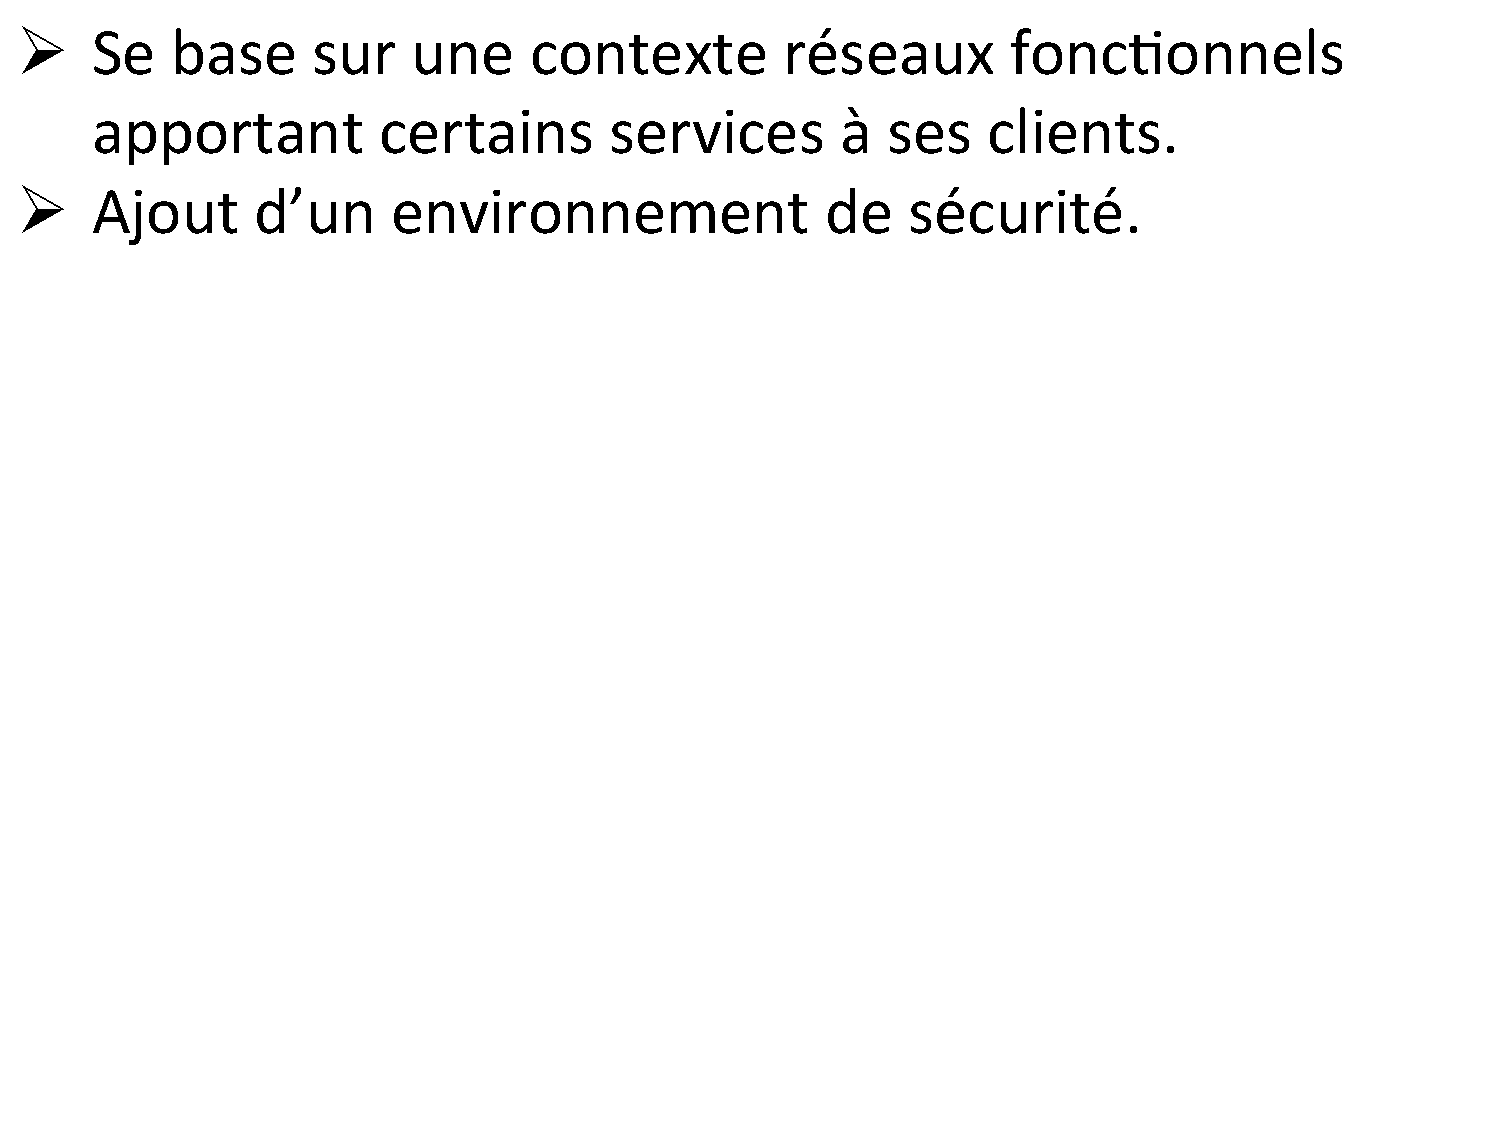
\includegraphics[scale=0.35]{slide1}}
\end{frame}

\begin{frame}[fragile]
\centerline{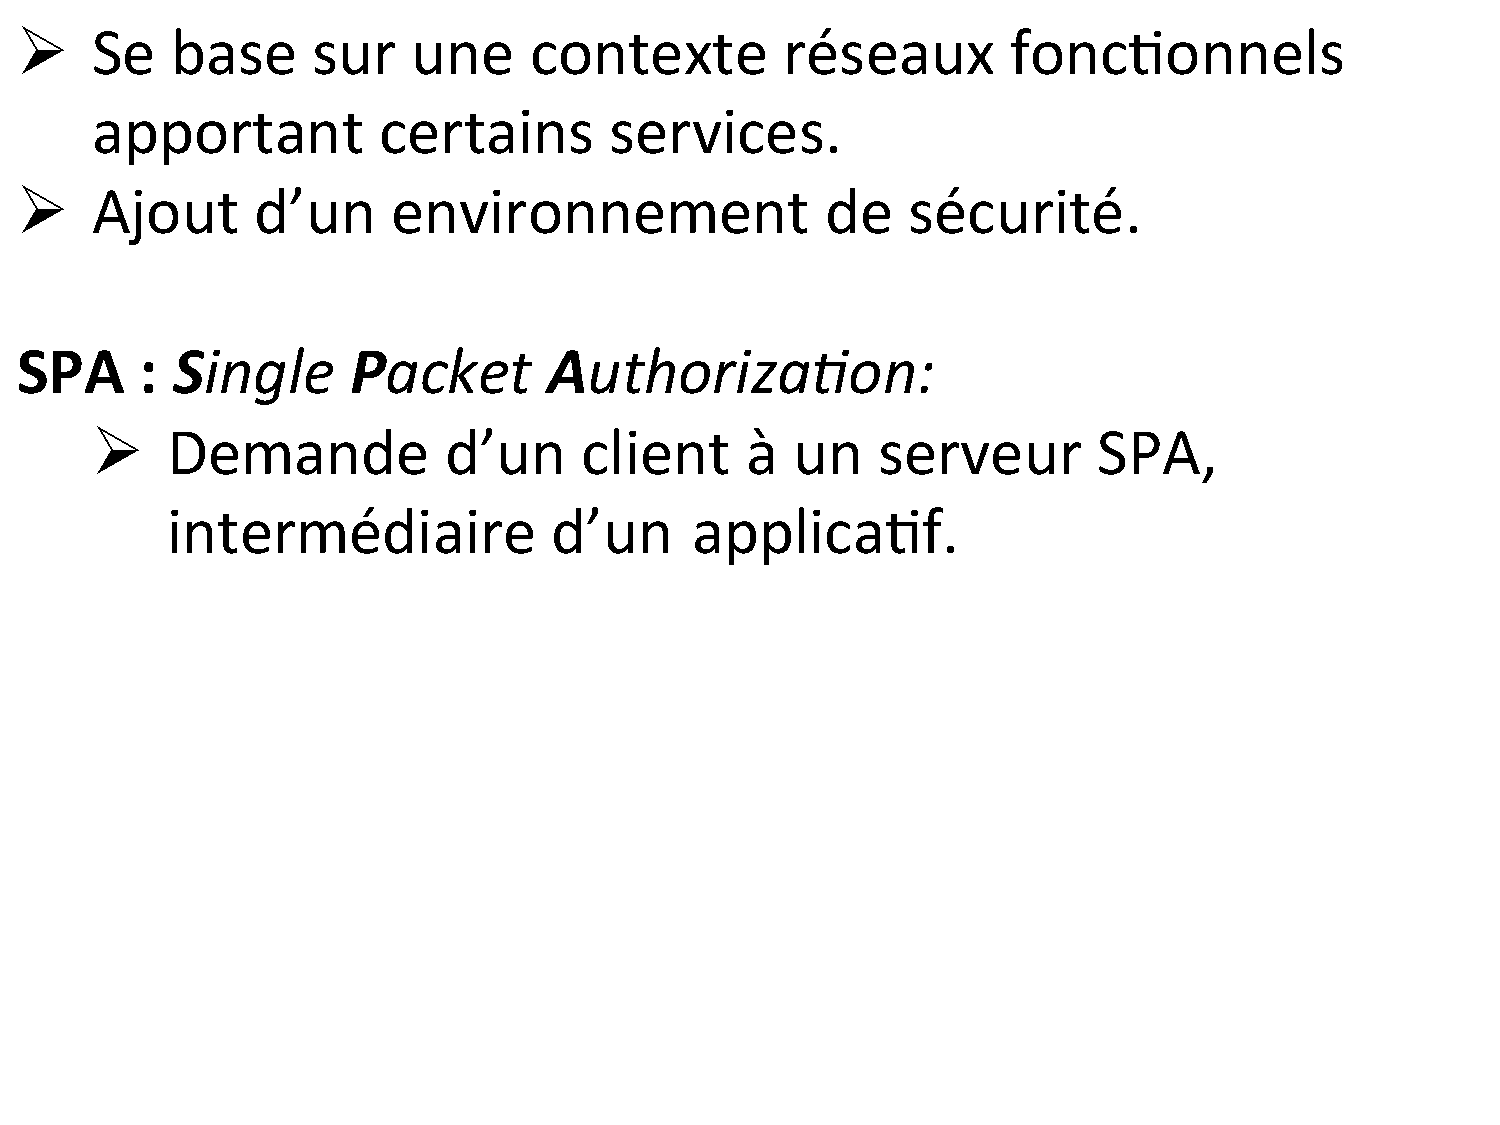
\includegraphics[scale=0.35]{slide2}}
\end{frame}

\begin{frame}[fragile]
\centerline{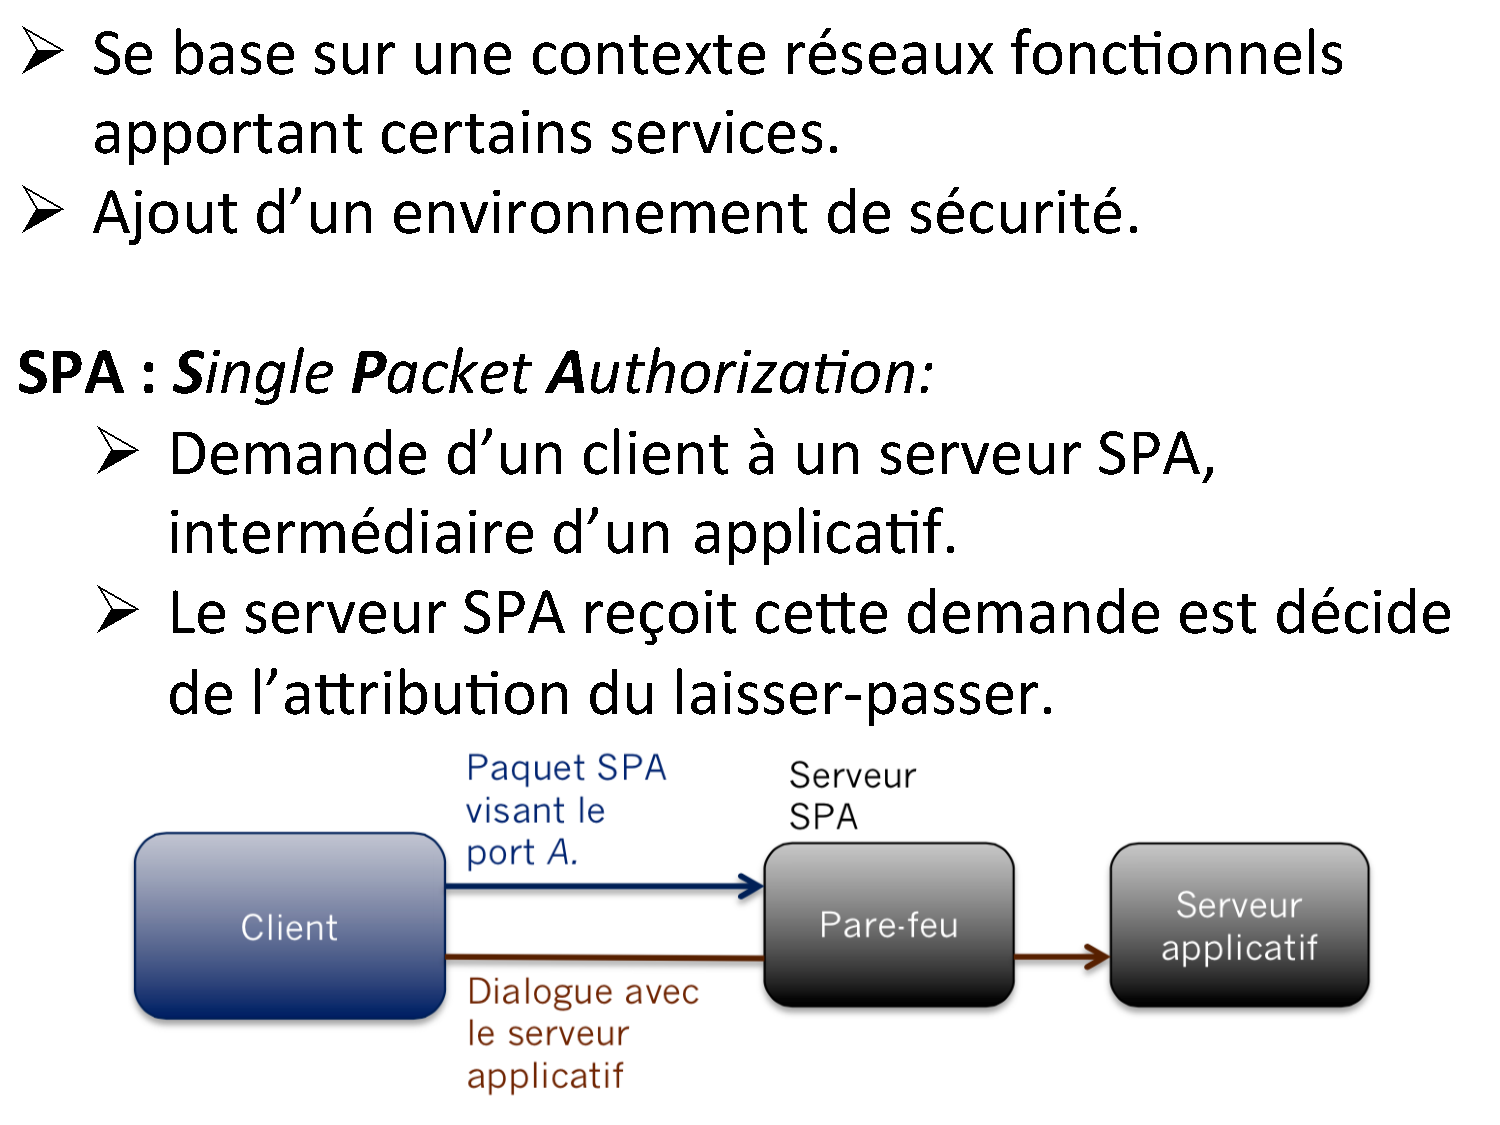
\includegraphics[scale=0.35]{slide3}}
\end{frame}

\begin{frame}[fragile]
\centerline{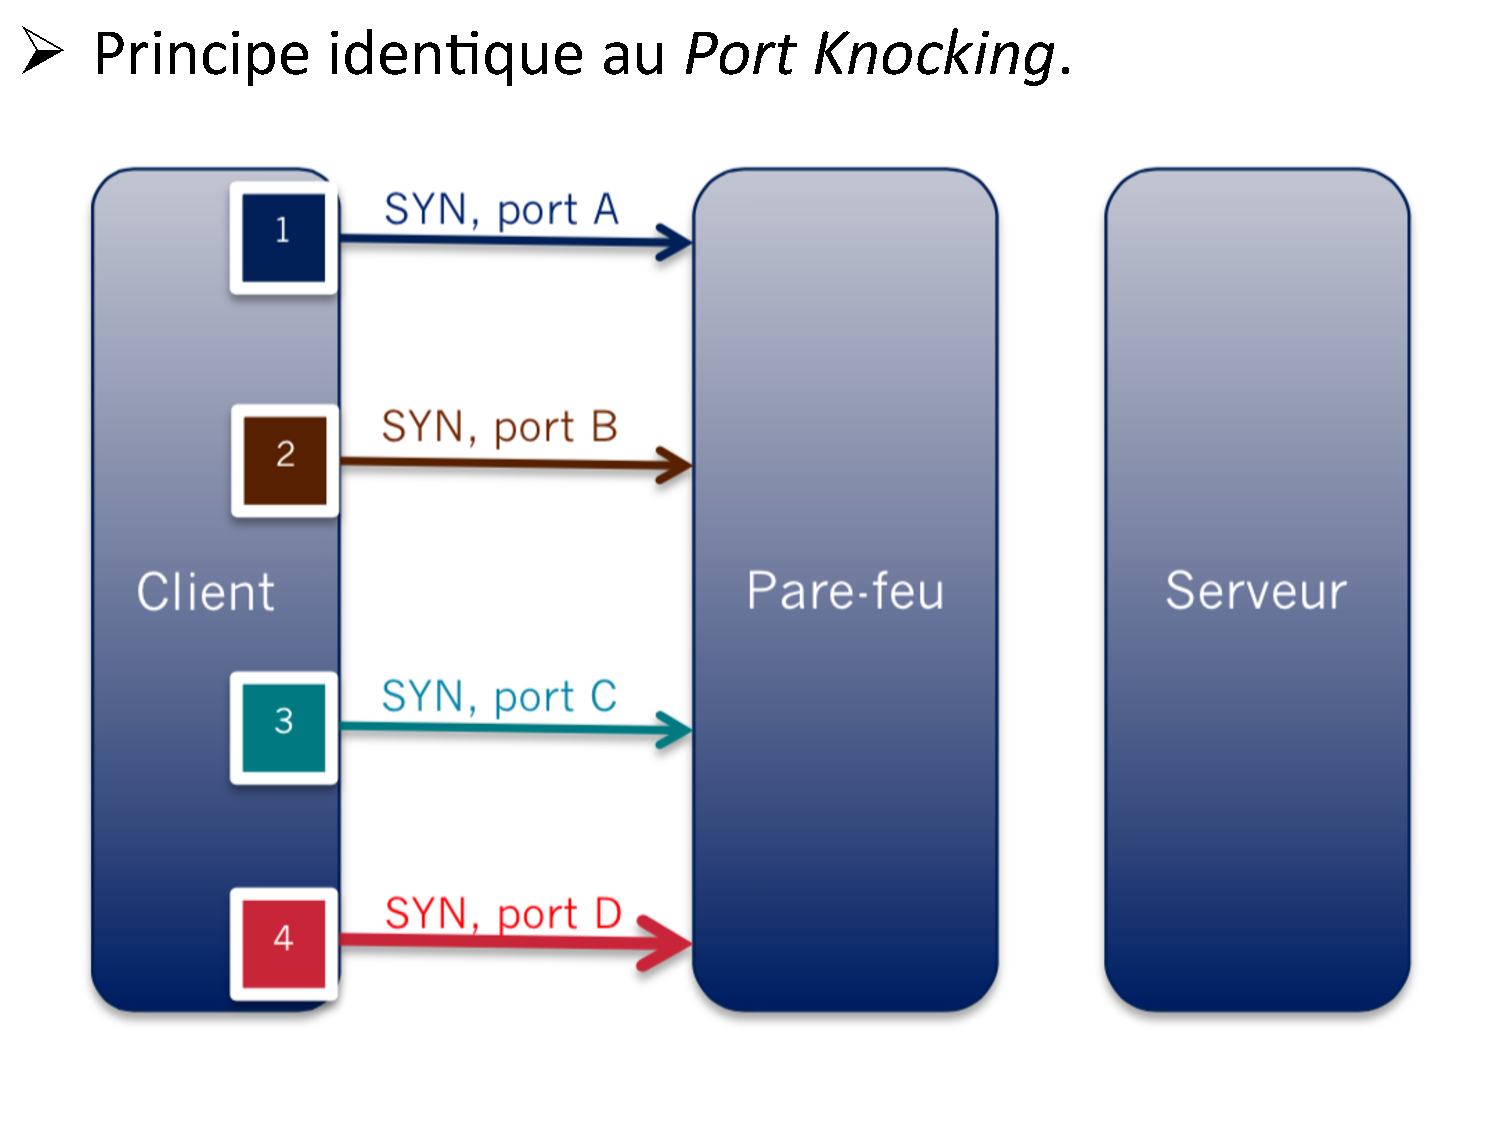
\includegraphics[scale=0.35]{slide4}}
\end{frame}

\begin{frame}[fragile]
\centerline{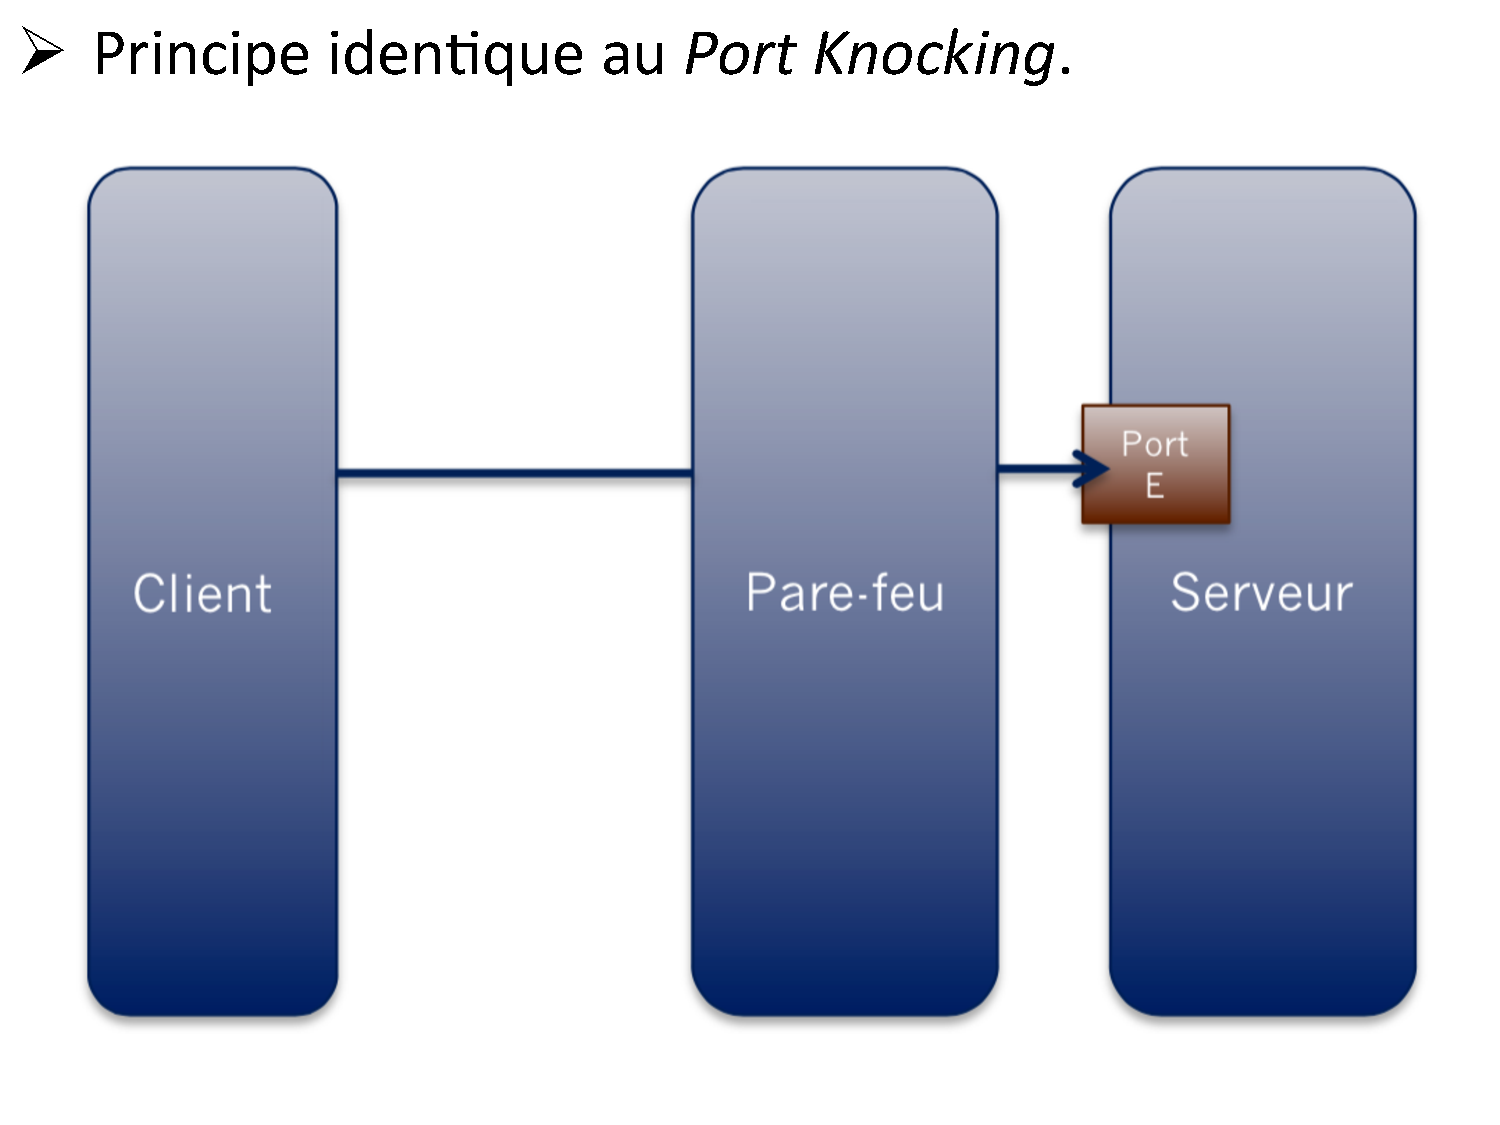
\includegraphics[scale=0.35]{slide5}}
\end{frame}


%%%%%%%%%%%%%%%%%%%%%%%%%%%%%%%%%%%%%%%%%%%%%%%%%%%%%%%%%%%%%%%%%%%%%%
\section{Génération}

\begin{frame}<handout:0>
  \frametitle{Plan}
  \tableofcontents[currentsection,subsectionstyle=hide]
\end{frame}

\begin{frame}[fragile]
\centerline{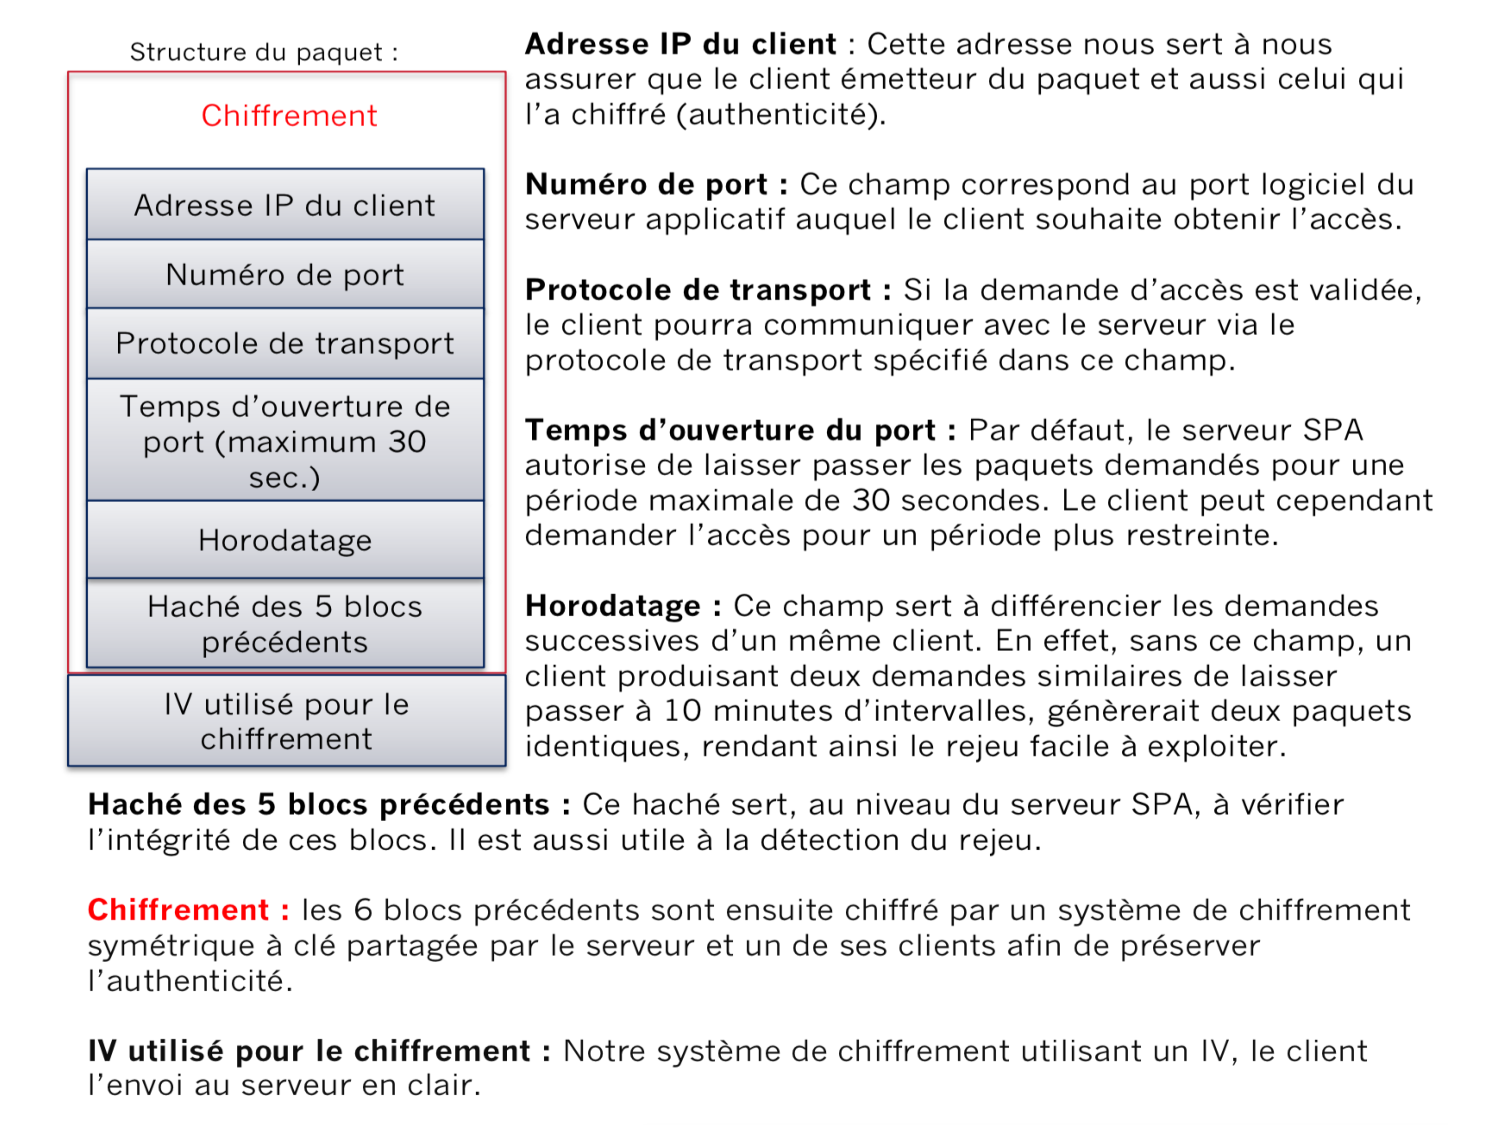
\includegraphics[scale=0.35]{slide6}}
\end{frame}



%%%%%%%%%%%%%%%%%%%%%%%%%%%%%%%%%%%%%%%%%%%%%%%%%%%%%%%%%%%%%%%%%%%%%%
\section{Protections contre le Rejeu}

\begin{frame}<handout:0>
  \frametitle{Plan}
  \tableofcontents[currentsection]
\end{frame}

\subsection{Horodatage}

\begin{frame}[fragile]
\frametitle{Horodatage}
\centerline{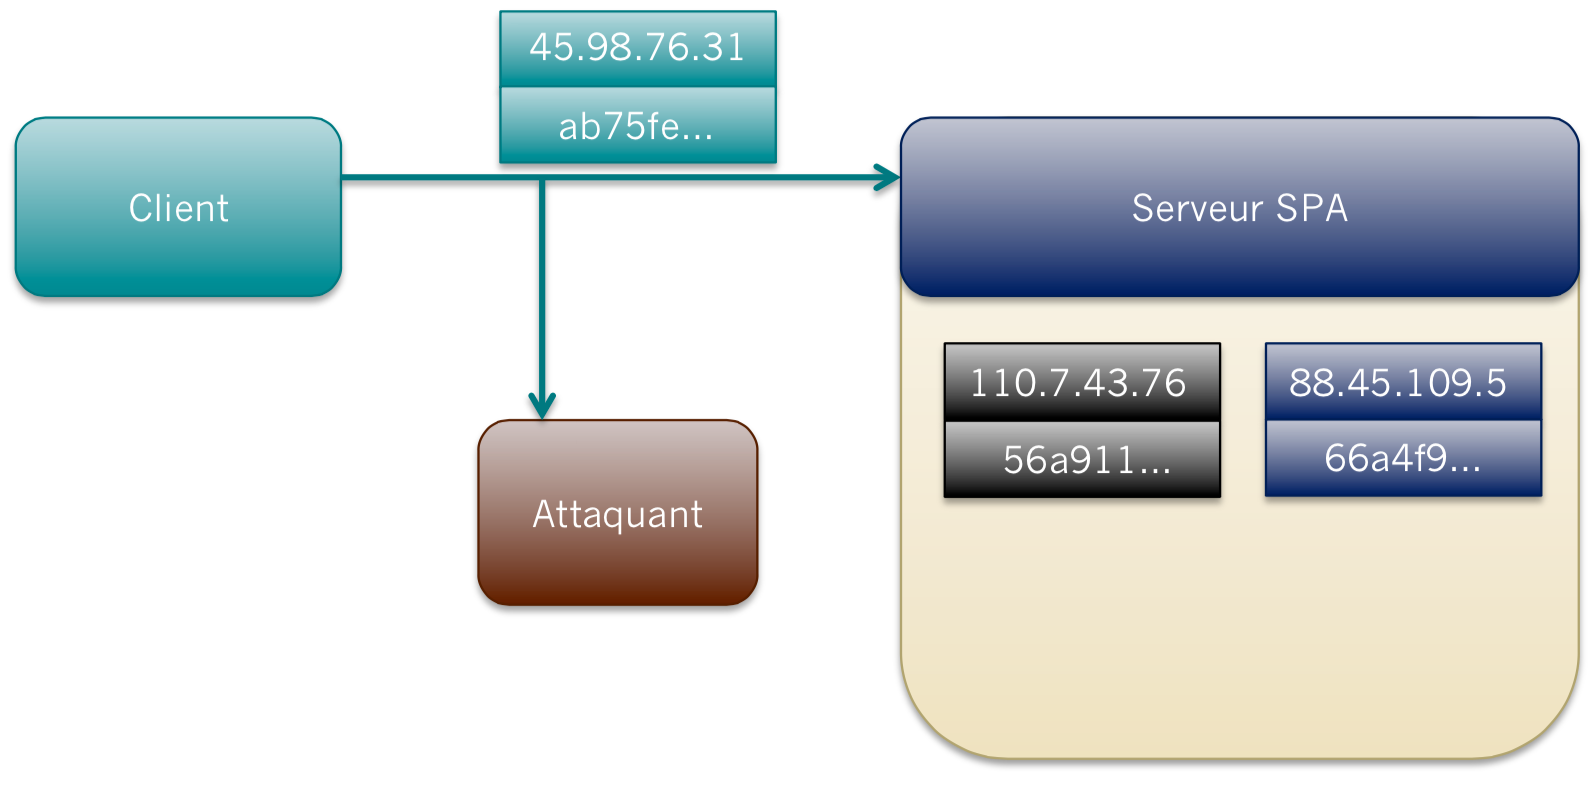
\includegraphics[scale=0.35]{horodatage_SPA1}}
\end{frame}

\begin{frame}[fragile]
\frametitle{Horodatage}
\centerline{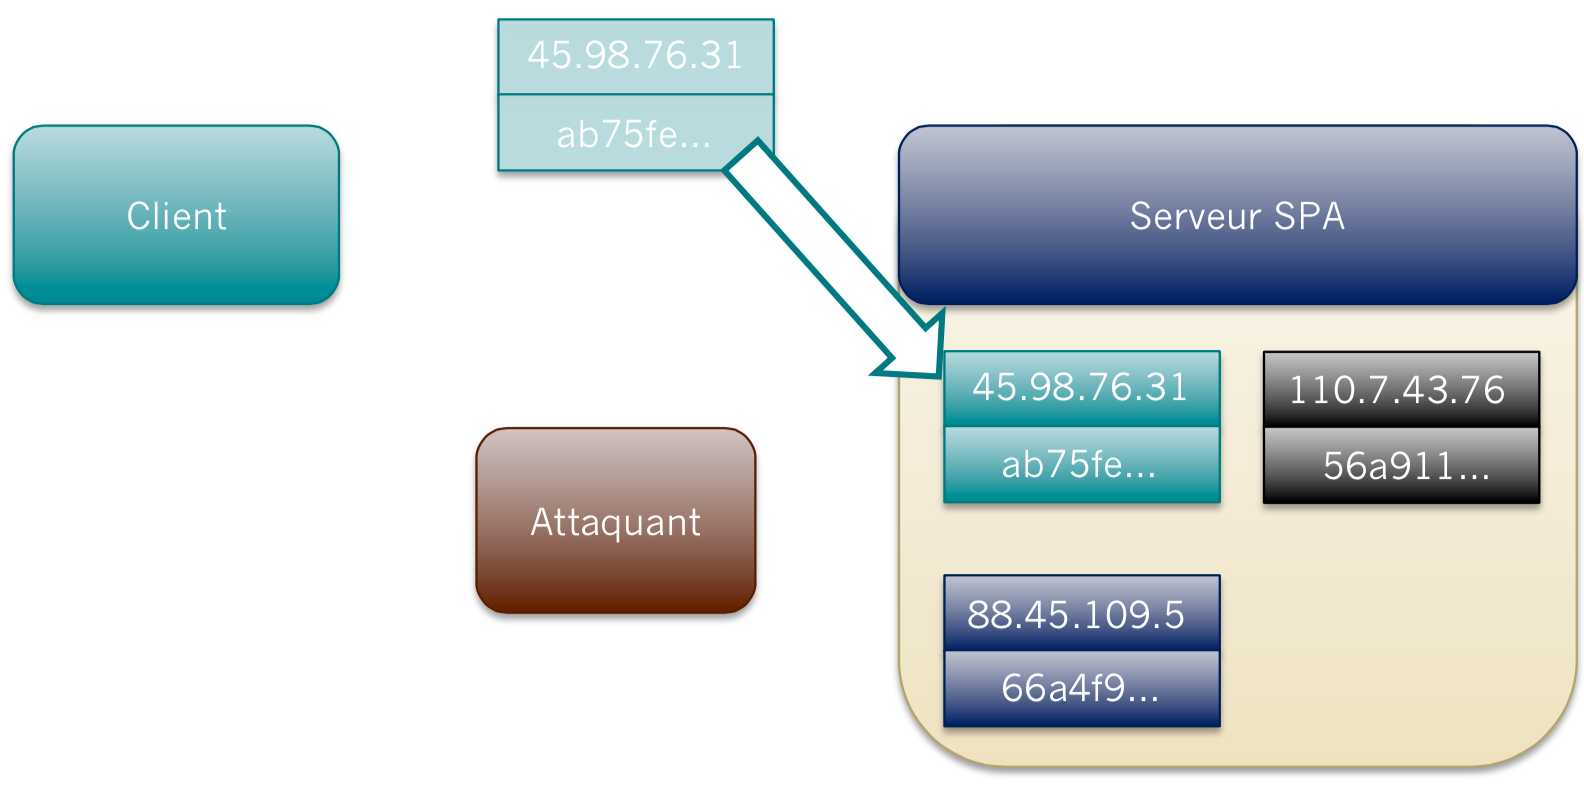
\includegraphics[scale=0.35]{horodatage_SPA2}}
\end{frame}

\begin{frame}[fragile]
\frametitle{Horodatage}
\centerline{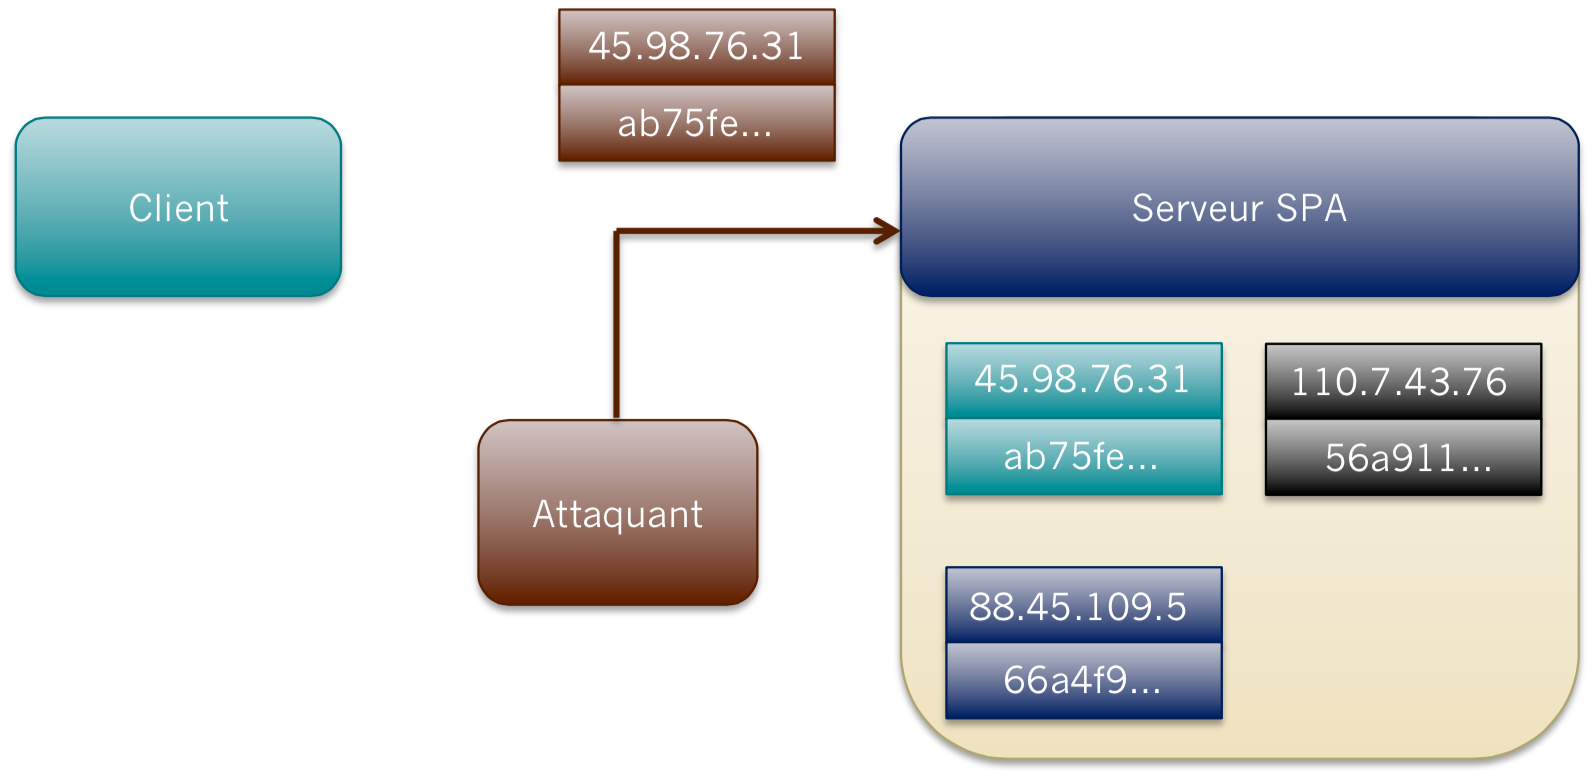
\includegraphics[scale=0.35]{horodatage_SPA3}}
\end{frame}

\subsection{Détection par les One Time Password}

\begin{frame}[fragile]
\frametitle{Détection par les One Time Password}
\centerline{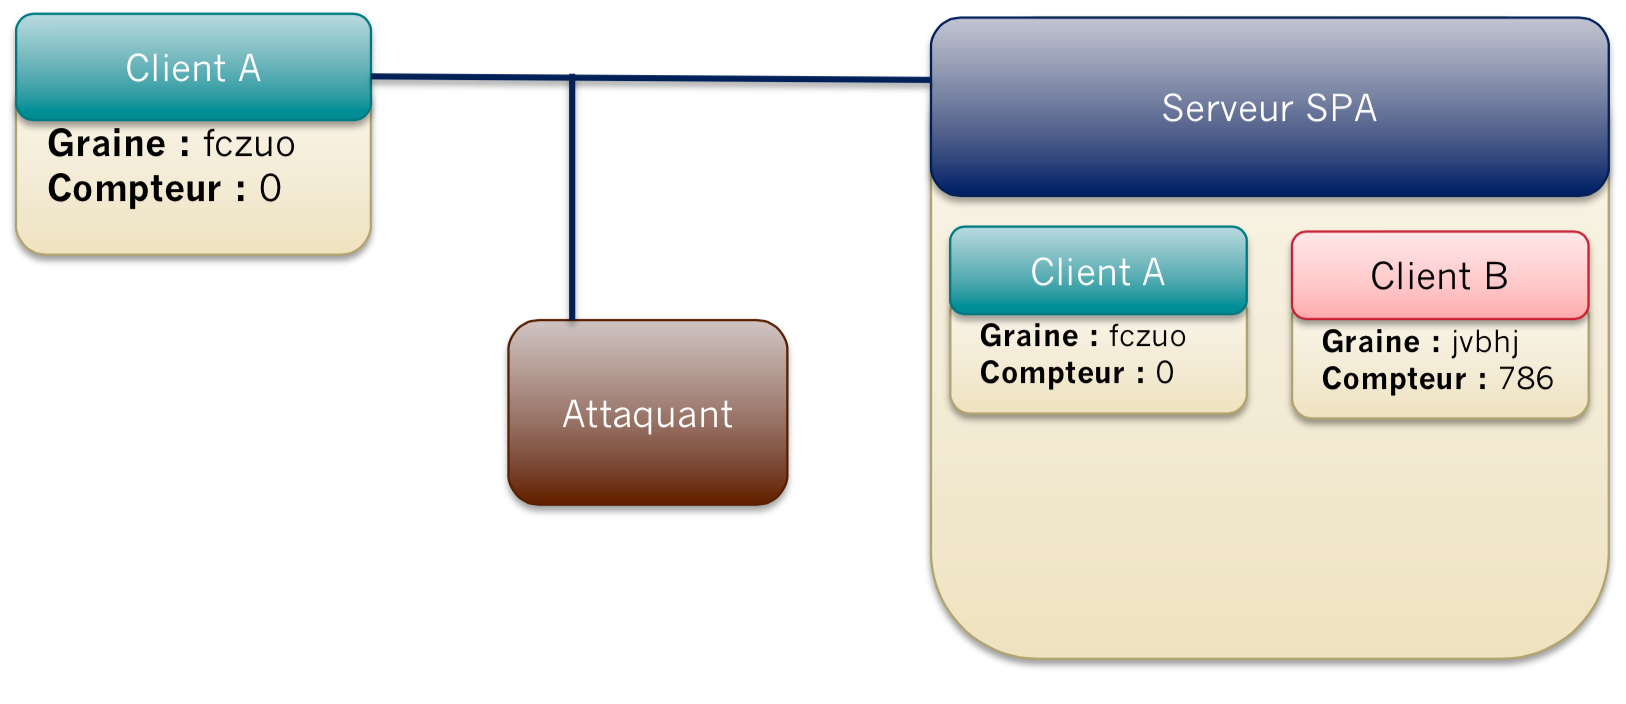
\includegraphics[scale=0.35]{OTP}}
\end{frame}

\begin{frame}[fragile]
\frametitle{Détection par les One Time Password}
\centerline{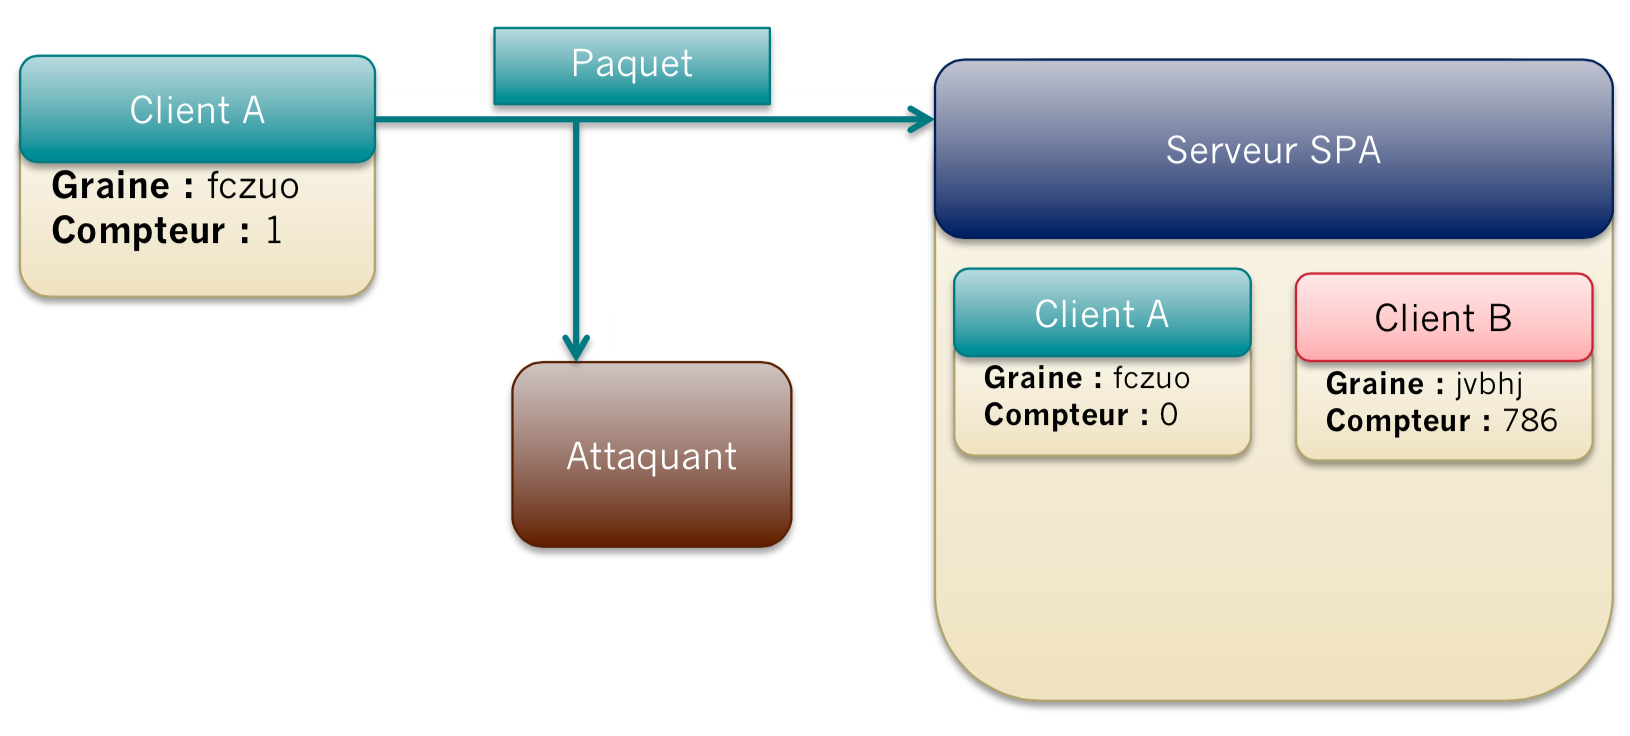
\includegraphics[scale=0.35]{OTP1}}
\end{frame}

\begin{frame}[fragile]
\frametitle{Détection par les One Time Password}
\centerline{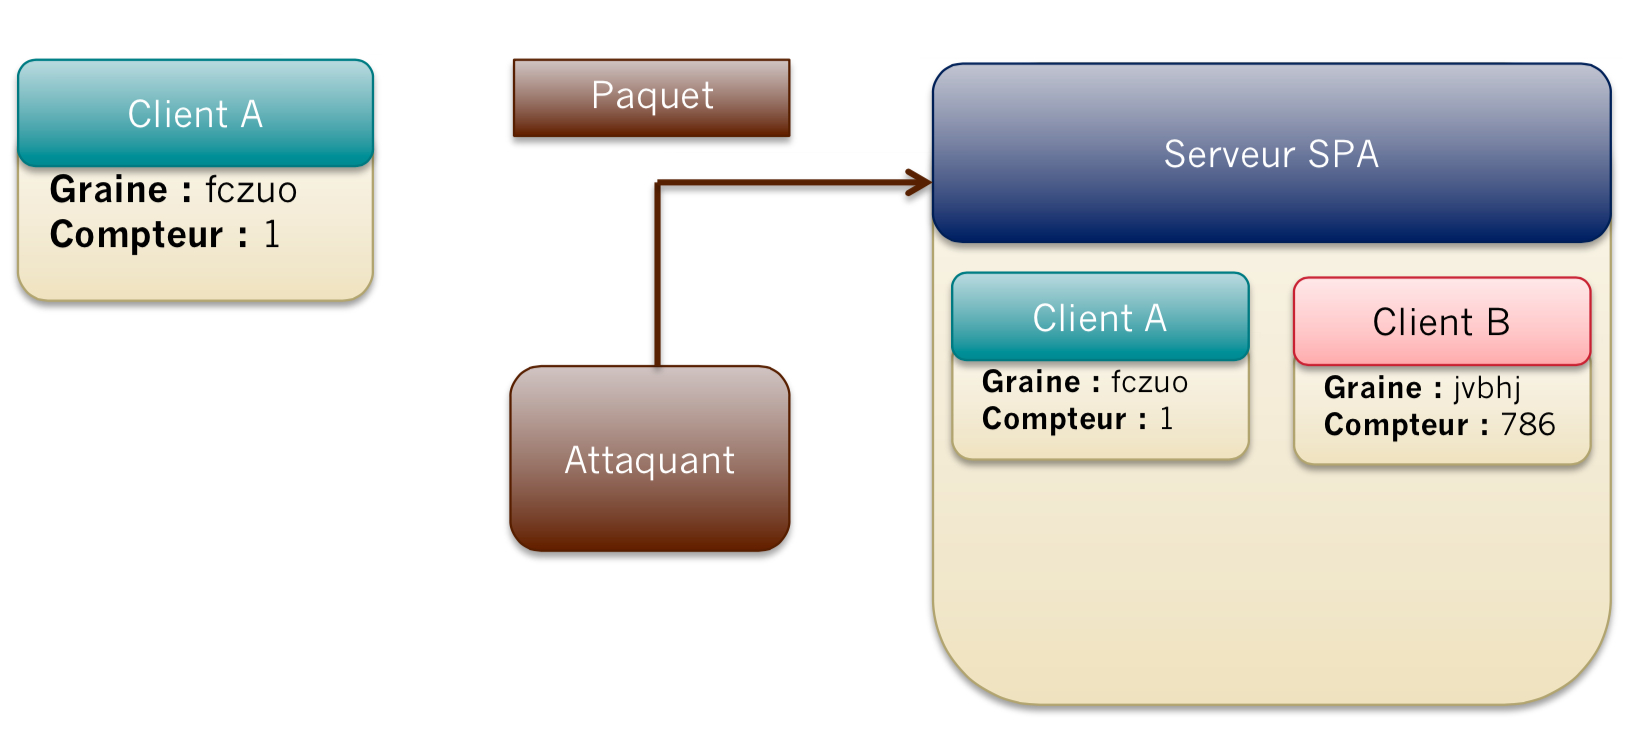
\includegraphics[scale=0.35]{OTP2}}
\end{frame}


%%%%%%%%%%%%%%%%%%%%%%%%%%%%%%%%%%%%%%%%%%%%%%%%%%%%%%%%%%%%%%%%%%%%%%
\section{Conclusion}

\begin{frame}<handout:0>
  \frametitle{Plan}
  \tableofcontents[currentsection,subsectionstyle=hide]
\end{frame}

\begin{frame}
\centerline{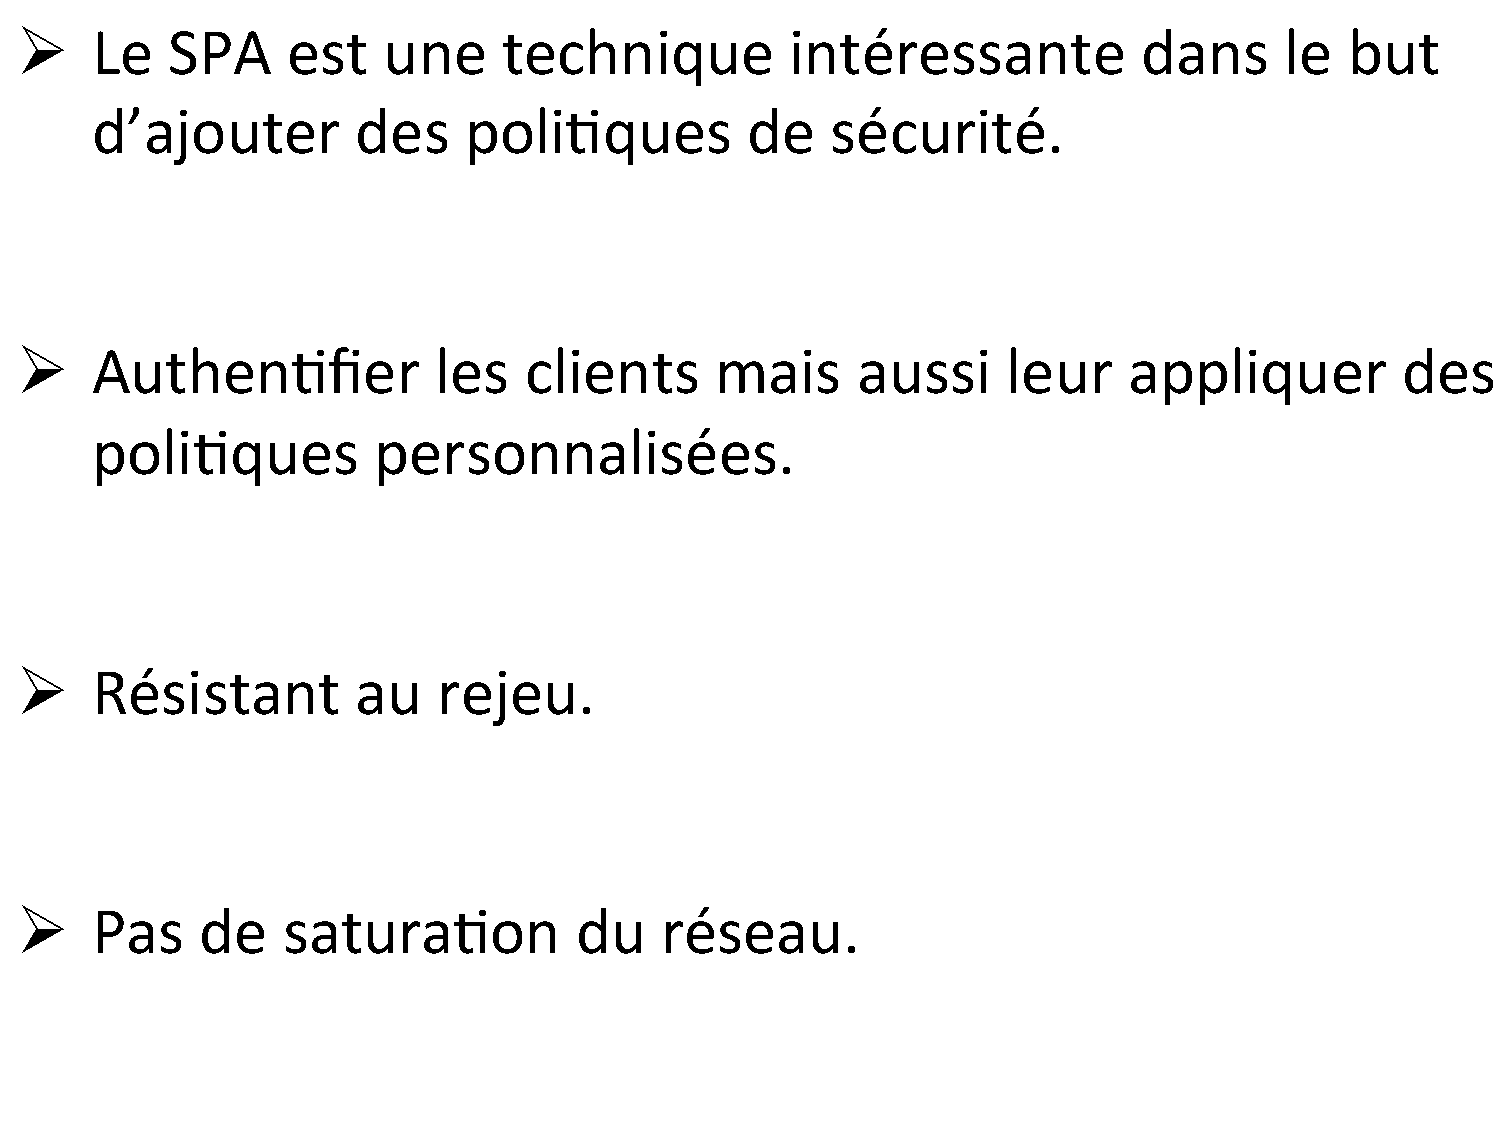
\includegraphics[scale=0.35]{conclu}}
\end{frame}

%%%%%%%%%%%%%%%%%%%%%%%%%%%%%%%%%%%%%%%%%%%%%%%%%%%%%%%%%%%%%%%%%%%%%%
\section{Références \& Lectures supplémentaires}

\begin{frame}<handout:0>
  \frametitle{Plan}
  \tableofcontents[currentsection,subsectionstyle=hide]
\end{frame}

\nocite{*}
\bibliographystyle{alpha}

\begin{frame}[allowframebreaks]
  \frametitle{Livres et références}
  \bibliography{bibliography}
\end{frame}

%%%%%%%%%%%%%%%%%%%%%%%%%%%%%%%%%%%%%%%%%%%%%%%%%%%%%%%%%%%%%%%%%%%%%%
\begin{frame}
  \vfill
  \centering
  \highlight{\Huge Questions~?}
  \vfill
\end{frame}
